%%%%%%%%%%%%%%%%%%%%%%%%%%%%%%%%%%%%%%%%%%%%%%%%%%%%%%%%%%%%%%%%%%%%%%%%%%%%%%%%%%%%%%%%%%%%%%%
%%%%%%%%%%%%%%%%%%%%%%%%%%%%%%%%%%%%%%%%%%%%%%%%%%%%%%%%%%%%%%%%%%%%%%%%%%%%%%%%%%%%%%%%%%%%%%%
\section{Experimental Setups}


%%%%%%%%%%%%%%%%%%%%%%%%%%%%%%%%%%%%%%%%%%%%%%%%%%%%%%%%%%%%%%%%%%%%%%%%%%%%%%%%%%%%%%%%%%%%%%%
\subsection{Datasets}

Six diverse datasets (of grayscale and color images, text and gene expressions) are used to show the application of our method to the real world dataset. (See Table.~\ref{tbl:dataset} for some samples of each dataset.)

\emph{DIGITS} is a subset of the optical recognition of handwritten digits dataset~\cite{kaynak1995methods} of 8x8 grayscale images.
\emph{COIL20} \cite{nene1996} is a dataset of 32x32 grayscale images of 20 rotated objects.
\emph{FASHION\_1K} contains 1000 grayscale images of size 28x28, sampled from Fashion-MNIST\cite{xiao2017/online} clothing dataset.
The grayscale images from three above datasets are normalized and used directly in the DR methods.

\emph{FASHION\_MOBILENET} dataset (\emph{FASH\_MOBI} for short) contains samples of seven most numerous classes from a subset of Fashion Product images dataset~\cite{fashionproduct}.
The MobileNet\cite{howard2017mobilenets} with pre-trained weights from ImageNet is used for feature extraction, a transfer learning technique that uses the representation of the learned network (trained on a large-scale image classification task) to extract meaningful features for new samples.
The last fully connected layer of the network is replaced by a global average pooling layer\cite[Sec.3.2]{lin2013network} to obtain the flattened output vector of 1280 dimensions.
To speed up the DR methods, PCA is then applied to take only 75 features.

\emph{5NEWS} dataset contains the text of 5 groups selected from the 20 Newsgroups dataset which are converted to a matrix of token counts via Term Frequency Inverse Document Frequency (TF-IDF) method.
The count vectors are then fed into Latent Dirichlet Allocation (LDA)~\cite{blei2003latent} model to extract 15 hidden topics, which are 15 features used for DR methods.

The open \emph{NEURON\_1K}~\cite{neuron1k} dataset contains 1301 brain cells from an E18 Mouse, processed and provided by 10X Genomics, a company who provides chromium single cell gene expression solution and releases several public genetic datasets.\footnote{https://www.10xgenomics.com/resources/datasets/, the datasets are licensed under the Creative Commons Attribution license.}
The processed data have 10 PCA features and labeled in 6 classes found by a graph-based clustering method.


\begin{table*}%[width=\textwidth,cols=6,pos=h]
\caption{Description of six selected datasets.}\label{tbl:dataset}
\begin{tabular}{m{2.2cm} m{5.4cm} m{7.4cm}}
\toprule
Dataset name & Samples & Description \\
\midrule

\emph{COIL20}
    & 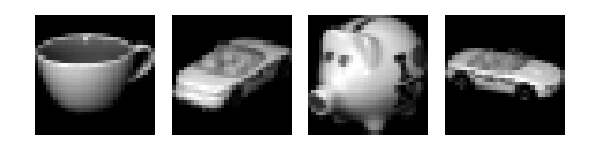
\includegraphics[width=\linewidth]{COIL20_samples}
    & 1440 grayscale images of size 32x32, belonging to 20 classes.
    The raw images of 1024 dimensions are used directly for the DR methods.\\

\emph{DIGITS}
    & 
\includegraphics[width=\linewidth]{DIGITS_samples}
    & 1797 grayscale images of size 8x8 of 10 digits.
    The raw images of 64 dimensions are used directly for the DR methods.\\

\emph{FASHION\_1K}
    & 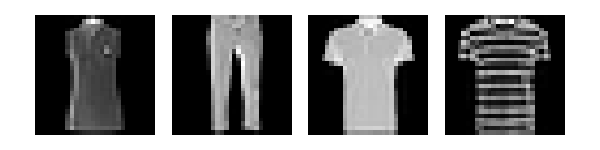
\includegraphics[width=\linewidth]{FASHION1000_samples}
    & 1000 grayscale images of size 28x28 of 10 classes, sampled from Fashion-MNIST dataset.
    The raw images of 768 dimensions are used directly for the DR methods.\\

\emph{FASH\_MOBI}
    & 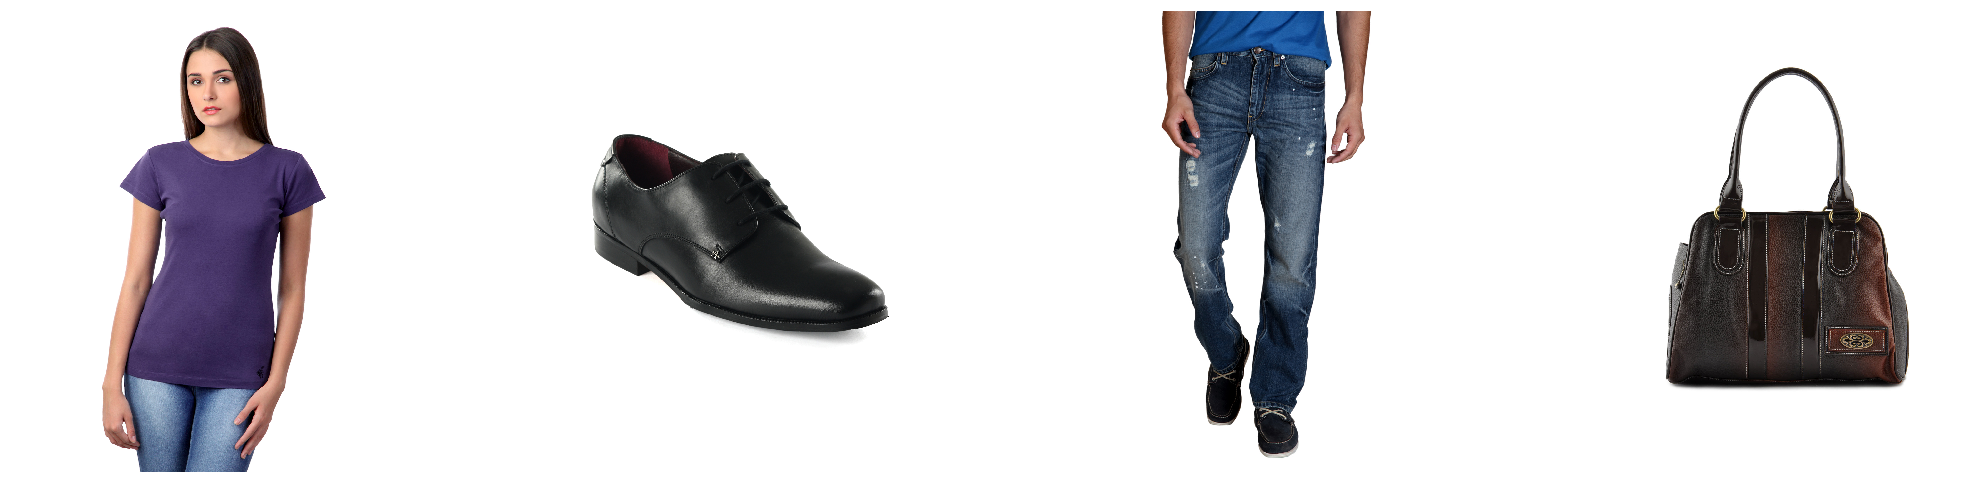
\includegraphics[width=\linewidth]{FASHION_PRODUCT_samples}
    & 1494 color images of various sizes belonging to 7 classes
    (\emph{'Bags', 'Bottomwear', 'Jewellery', 'Sandal', 'Shoes', 'Topwear', 'Watches'}),
    sampled from Fashion Product images dataset.\\

\emph{5NEWS}
    & 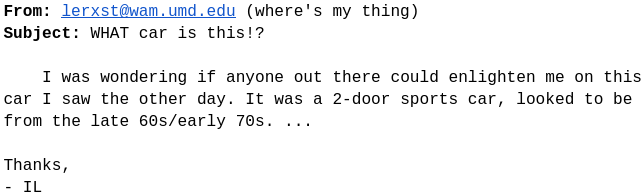
\includegraphics[width=\linewidth]{20NEWS5_samples}
    & 5 groups of 2957 emails selected from 20Newsgroups dataset,
    including \emph{'rec.autos', 'rec.sport.baseball','sci.crypt', 'sci.space', 'comp.sys.mac.hardware'}. \\

\emph{NEURON\_1K}
    &
    & 1301 brain cells from a combined cortex, hippo-campus and sub-ventricular zone of an E18 mouse. \\

\bottomrule
\end{tabular}
\end{table*}

%%%%%%%%%%%%%%%%%%%%%%%%%%%%%%%%%%%%%%%%%%%%%%%%%%%%%%%%%%%%%%%%%%%%%%%%%%%%%%%%%%%%%%%%%%%%%%%
\subsection{Constraint Generation}

The input for our proposed constraint preserving scores is ensemble of constraints in form of similar links and dissimilar links.
However, it is hard to control the quality of the constraints.
For example, a similar link between two different data points is not expected.
The number of constraints each type also affects the stability of the score.
In order to correctly evaluate the score function, we do not use the pairwise constraints directly, but use a small subset of instances with labels to generate the constraints instead.

Give a dataset of $C$ classes, for each class we take randomly $k$ labeled instances to generate the constraints.
Suppose that the number of instances in each class is larger than $k$ ($k$ is usually very small).
A similar link is formed by choosing a random pair from $k$ labeled instances of a class.
The number of all possible similar links is given by:
\begin{equation}\label{equ:n-sim-link}
n_{sim\_link} = C {k \choose 2} = \frac{1}{2} C k (k-1)
\end{equation}
A dissimilar link is formed by first choosing two different classes among $C$ classes (${C \choose 2}$ ways),
then choosing a pair of two instances from these two chosen classes ($k^2$ pairs).
The number of all possible dissimilar links is given by:
\begin{equation}\label{equ:n-dis-link}
n_{dis\_link} = {C \choose 2} k^2 = \frac{1}{2} C (C-1) k^2
\end{equation}

Intuitively, the more labeled points we had, the more constraints are generated and the more stable the $f_{score}$ is.
We will show in the next section the experimental setup for the proof of concept.
Indeed, with 10 labeled points for each of 10 classes of the DIGITS dataset for example, they are around 5.6\% of total labels but can generate 450 similar links and 4500 dissimilar links.

%%%%%%%%%%%%%%%%%%%%%%%%%%%%%%%%%%%%%%%%%%%%%%%%%%%%%%%%%%%%%%%%%%%%%%%%%%%%%%%%%%%%%%%%%%%%%%%
\subsection{Proof of Concept}
We design the experiments to answer the research questions concerning to the stability (Section~\ref{sec:result:stability}) and flexibility (Section~\ref{sec:result:flexibility}) of the proposed score and the application of BayOpt to $f_{score}$ (Section~\ref{sec:result:bo}).
As a proof of concept, we create a grid of hyperparameters for t-SNE, LargeVis and UMAP, and then calculate $f_{score}$ for each embedding corresponding to each combination.
The hyperparameters are sampled in natural logarithmic scale (log-scale) since we want to focus on the values which are not too large.
In the case of t-SNE and LargeVis, the grid is an integer vector of perplexity values from 2 to $N/3$ in log-scale, in which $N$ is the number of instances of the dataset.
In the case of UMAP, the two dimensional grid is all combinations of its two hyperparameters.
The first dimension is an integer vector of $n\_neighbor$ values from 2 to $N/3$ in log-scale.
The second dimension is a vector of 10 real values of $min\_dist$ from 0.001 to 1.0 in log-scale.
This grid helps us to analyze the behavior of the proposed $f_{score}$ w.r.t. different combinations of hyperparameters.
The $f_{score}$ values on this grid are also used as ground-truth score values to evaluate the prediction of BayOpt approach.
It is important to note that, the creation of this grid is computationally expensive and increases exponentially with the number of hyperparameters.
The grid is only used as proof of concept to evaluate the reliability of the BayOpt approach on the proposed score.
As shown in the next section, BayOpt approach solves the scalability problem efficiently, in which only dozens of evaluations are required to find the best hyperparameters for all experimented datasets.

For all hyperparameter tuning tasks under BayOpt framework, we prefer the exploration strategy to make sure we can discover the largest as possible the parameter space.
Three technical points that guarantees the accuracy in predicting the best hyperparameters the quick convergence of BayOpt in our experiments are follows.
(1) The hyperparameters are sample in natural logarithmic domain to focus the computation on not-so-large values, which are usually used in practice.
(2) Expected Improvement (EI) acquisition function is used as a surrogate function in the underlying Gaussian Process (GP) model of BayOpt.
The exploration strategy is set using a large value of parameter $\xi$ of EI, which controls the trade-off between global search (exploration) and local optimization (exploitation).
All our experiments for all datasets are run with $\xi=0.1$ without any effort to tune this parameter.
(3) Since there is always a small variance in the score value, there is some noise in the observations (the $f_{score}$ values) for BayOpt and the underlying kernel of GP model must be aware of this noise.
This can be done by adding the small values to the diagonal of the GP's kernel matrix.
This reminds us to always take into account not only the noise in the observation but also the uncertainty in the prediction of the GP model.

%%%%%%%%%%%%%%%%%%%%%%%%%%%%%%%%%%%%%%%%%%%%%%%%%%%%%%%%%%%%%%%%%%%%%%%%%%%%%%%%%%%%%%%%%%%%%%%
%%%%%%%%%%%%%%%%%%%%%%%%%%%%%%%%%%%%%%%%%%%%%%%%%%%%%%%%%%%%%%%%%%%%%%%%%%%%%%%%%%%%%%%%%%%%%%%
\section{Stability of Constraint Preserving Score}\label{sec:result:stability}

The proposed constraint preserving score is a function of the pairwise constraints $f_{score}(\mathcal{S}, \mathcal{D})$ which are generated automatically from the input labeled instances.
The first question is that, how does $f_{score}$ vary with respect to different number of labeled instances?
Moreover, with a fixed number of labeled instances, we can generate different set of pairwise constraints.
The second question is, with different set of constraints generated from the same fixed number of labeled instances, is $f_{score}$ stable?
In order to answer these two questions, $f_{score}$ is evaluated for five different numbers of labeled instances (3, 5, 10 and 15).
The labeled points are independent and not accumulated, i.e., the 5 labeled instances in the second setting do not contain the 3 labeled instances in the first setting.
$f_{score}$ is a function of pairwise constraints, which can vary while the number of constraints is fixed.
Thus, in each setting with a fixed number of labeled instances, 20 different set of pairwise constraints are generated.
We will show the average value and the standard deviation of $f_{score}$.
For t-SNE and LargeVis, $f_{score}$ is evaluated for different perplexity.
For UMAP, $f_{score}$ is evaluated for different \emph{n\_neighbors} while fixing the second hyperparameter \emph{min\_dist} to its default value of 0.1.
The \emph{n\_neighbors} in UMAP plays the same role as perplexity in t-SNE, which indicates the expected number of neighbors of each points.

\begin{figure}%[pos=h]
\begin{subfigure}[b]{0.3\linewidth}
     \centering
     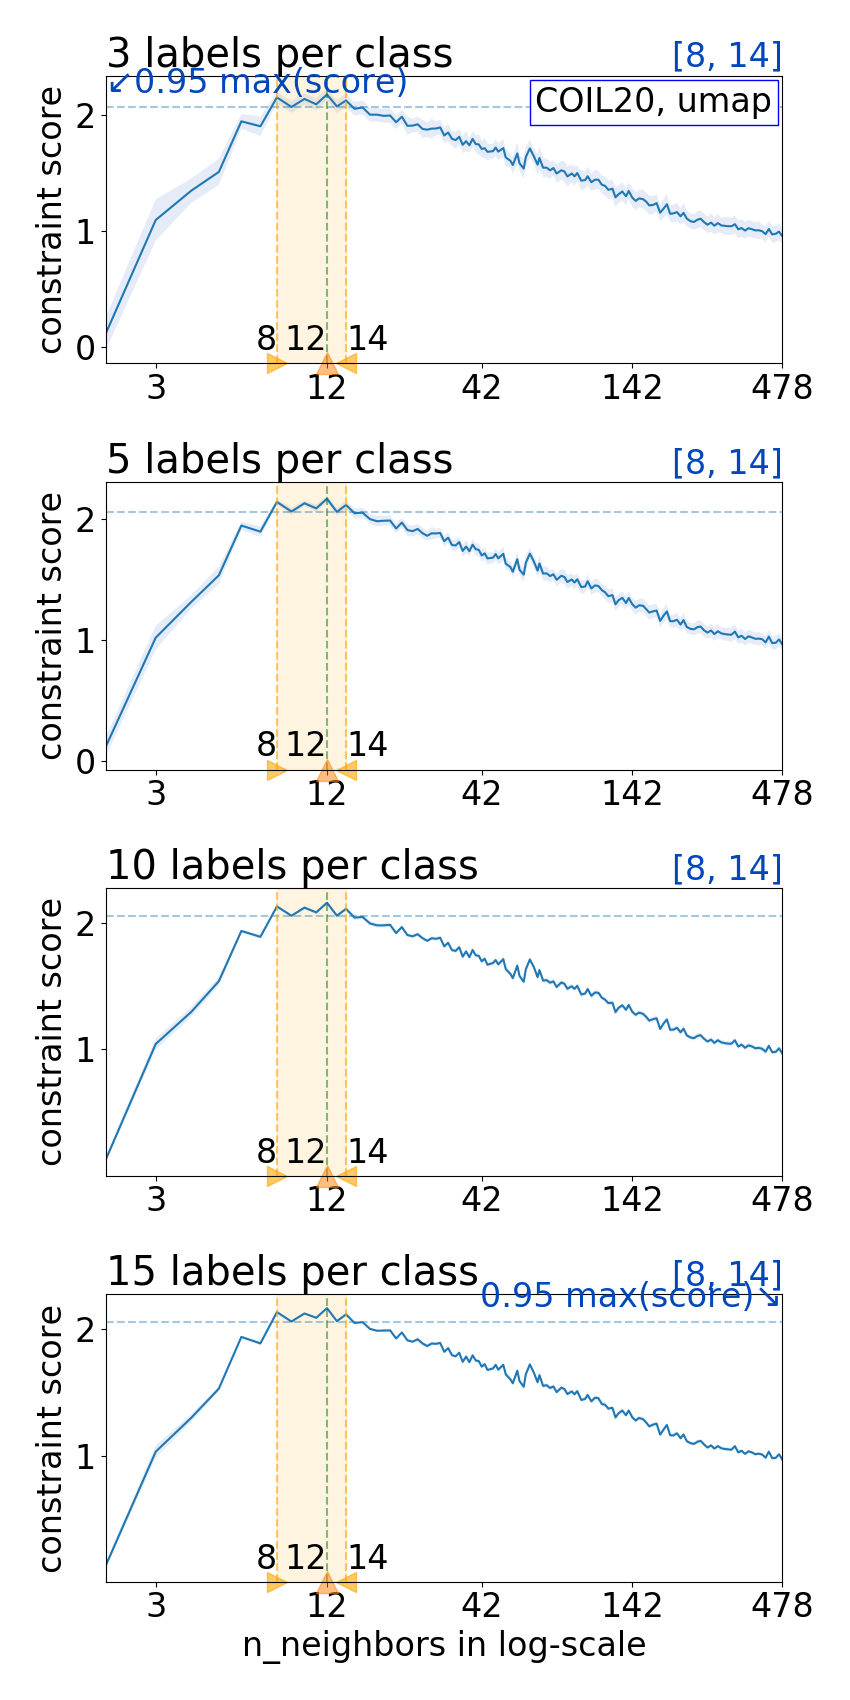
\includegraphics[width=\linewidth]{COIL20_umap_scores}
     \caption{UMAP}
\end{subfigure}
\hfill
\begin{subfigure}[b]{0.3\linewidth}
     \centering
     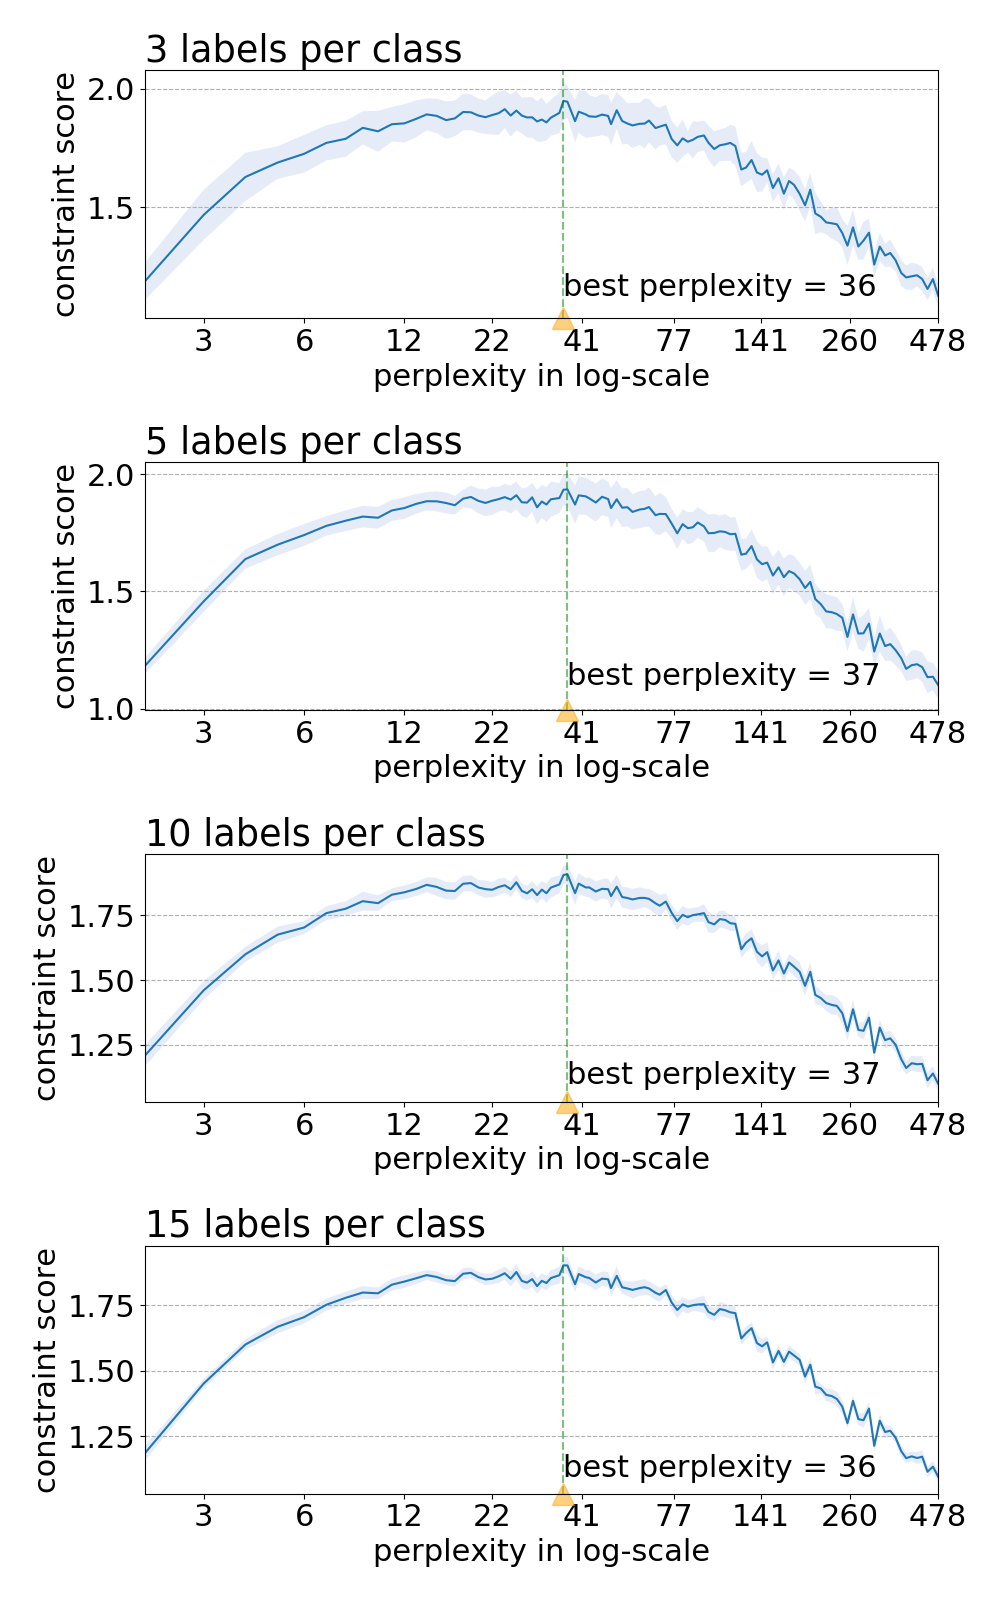
\includegraphics[width=\linewidth]{COIL20_tsne_scores}
     \caption{t-SNE}
\end{subfigure}
\hfill
\begin{subfigure}[b]{0.3\linewidth}
     \centering
     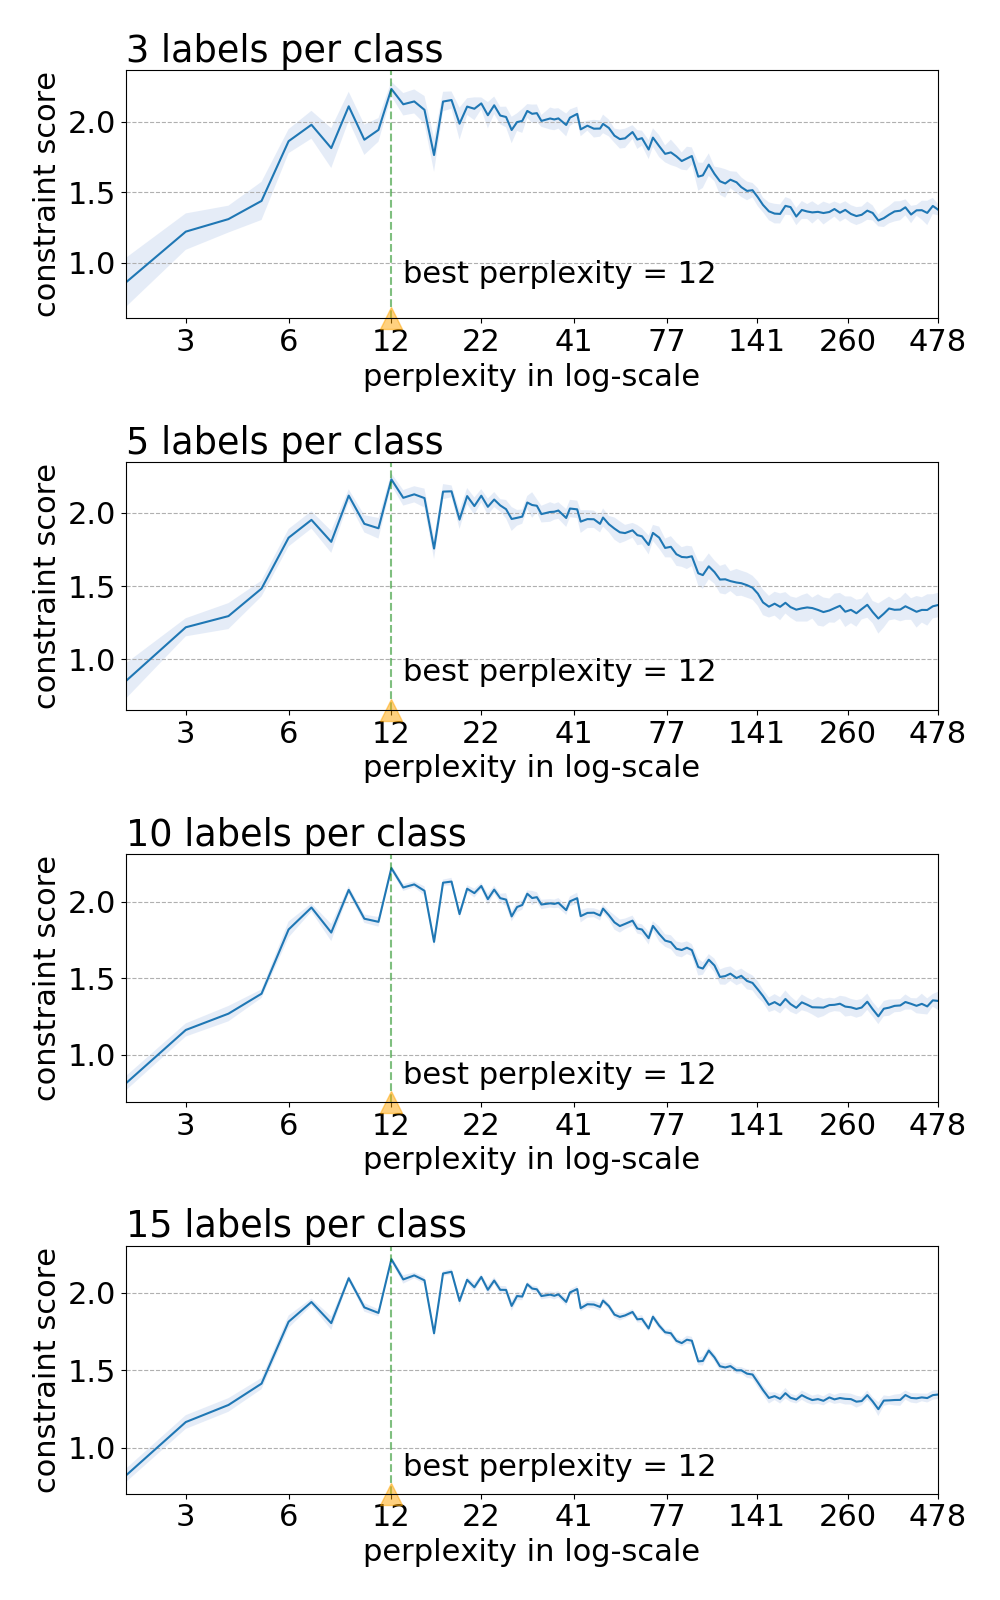
\includegraphics[width=\linewidth]{COIL20_largevis_scores}
     \caption{LargeVis}
\end{subfigure}
\caption{Stability of the constraint preserving scores with UMAP, t-SNE and LargeVis for COIL20 dataset.
The filled region highlights the best range of hyperparameters which make the score value superior to 96\% of maximum score value.}
\label{fig:score:stability:COIL20}
\end{figure}

Fig.~\ref{fig:score:stability:COIL20} shows the score for \emph{COIL20} dataset with the embeddings of UMAP (with fixed \emph{min\_dist} of 0.1), t-SNE and LargeVis.
The values of hyperparameter (perplexity and \emph{n\_neighbor}) are shown in natural logarithmic scale.
The following findings are shown for \emph{COIL20} dataset but also true for others experimented datasets.
First, the proposed constraint preserving score has the form like a convex function.
$f_{score}$ is not smooth but it can distinguish the characteristic of the embeddings of all DR methods.
$f_{score}$ increases when the number of neighbors increases, reaches to its maximum value, and decreases when perplexity/\emph{n\_neighbors} is too large.
Second, when the number of labeled instances increase, $f_{score}$ is more stable since the variance (presented by the standard deviation) dramatically decrease.
Third, the score is calculated only for discrete samples of the hyperparameter, there is always distortion in the value of $f_{score}$.
Selecting the best hyperparameter corresponding to the maximum score value may be not a reasonable choice since there are several hyperparameters that give almost the same score.
It can be better if we select a range of best hyperparameters that have the score value larger than a threshold, 96\% the maximum score value for example.
Fig.~\ref{fig:score:stability:COIL20} demonstrates that the best hyperparameters ranges are consistent w.r.t. different number of labeled instances.

In the case of LargeVis, there are the \emph{flat} regions where the score does not change too much.
The reason is that, LargeVis is designed for large dataset and thus when being applied to the medium-sized datasets as in our experiments, the impact of perplexity is not important.
In contrast, t-SNE and UMAP are very sensitive to its hyperparameters, especially in the case of very small and very large number of neighbors.
Intuitively, when the number of neighbors is small, the points are not grouped in the visualization.
The similar constraints are unlikely preserved while the dissimilar constraints have more change to be preserved since the points stay away from each other.
In this case $f_{score}(\mathcal{S})$ is very low and $f_{score}(\mathcal{D})$ is high, that makes $f_{score}$ low.
Inversely, when the number of neighbors is large, every point is neighbor to each other, which make the visualization a big cluster.
In this case, the similar constraints are likely preserved while the dissimilar constraints are note, that make $f_{score}(\mathcal{S})$ high and $f_{score}(\mathcal{D})$ low.

In summary, the local structures (neighborhood information) of the dataset are presented by the small groups in the visualization.
The clearer these groups are highlighted, the more likely the similar constraints of the points within groups and the dissimilar constraints of the points between different groups are preserved.
The proposed score has well captured this characteristic,  it reaches to the high values only when both the similar and dissimilar constraints are preserved.
Thus $f_{score}$ can be used to quantitatively evaluate the quality of the visualization and can be comparable to the state of the art quality metrics.
Moreover, for all selected datasets, the above experimental results indicated that {\bf 10 labeled instances per class} is sufficient for obtaining a stable score.
Since LargeVis is not sensitive to its perplexity, we will tune hyperparameters for t-SNE and UMAP on all six selected dataset using BayOpt approach.
The results are presented in the next section.


%%%%%%%%%%%%%%%%%%%%%%%%%%%%%%%%%%%%%%%%%%%%%%%%%%%%%%%%%%%%%%%%%%%%%%%%%%%%%%%%%%%%%%%%%%%%%%%
%%%%%%%%%%%%%%%%%%%%%%%%%%%%%%%%%%%%%%%%%%%%%%%%%%%%%%%%%%%%%%%%%%%%%%%%%%%%%%%%%%%%%%%%%%%%%%%
\section{Application of BayOpt on $f_{score}$}\label{sec:result:bo}
BayOpt is widely used for hyperparameter tuning problem when the target function is well-defined.
BayOpt is a general framework which can work with any complex target function like $AUC_{log}RNX$ score or BIC-based score function.
In practice, $AUC_{log}RNX$ does not always work well with UMAP's embedding, especially in the case of tuning two UMAP's hyperparameters at the same time.
BIC-based score is tiered to t-SNE and does not work for other DR methods.
$f_{score}$ is designed to be independent to the DR methods and to be flexible to the input constraints.
In this section, the input constraints are generated from 10 labeled instances in each class for any given dataset.
$f_{score}$, $AUC_{log}RNX$ and BIC-based scores are compared in both tasks of tuning one hyperparameter for t-SNE (Sec~\ref{sec:x}) and tuning two hyperparameters for UMAP (Sec~\ref{sec:y}).
In the next section, a different set of labeled points which does not base on the available class labels of the dataset is used.
$f_{score}$ which is flexible by design, can find the best visualization w.r.t. the new constraints.
This task can not be archived by $AUC_{log}RNX$ or BIC-based score.

%%%%%%%%%%%%%%%%%%%%%%%%%%%%%%%%%%%%%%%%%%%%%%%%%%%%%%%%%%%%%%%%%%%%%%%%%%%%%%%%%%%%%%%%%%%%%%%
\subsection{BayOpt for Tuning One Parameter of t-SNE}
\begin{figure}[]%[pos=h]
    \begin{subfigure}[b]{.46\linewidth}
        \centering
        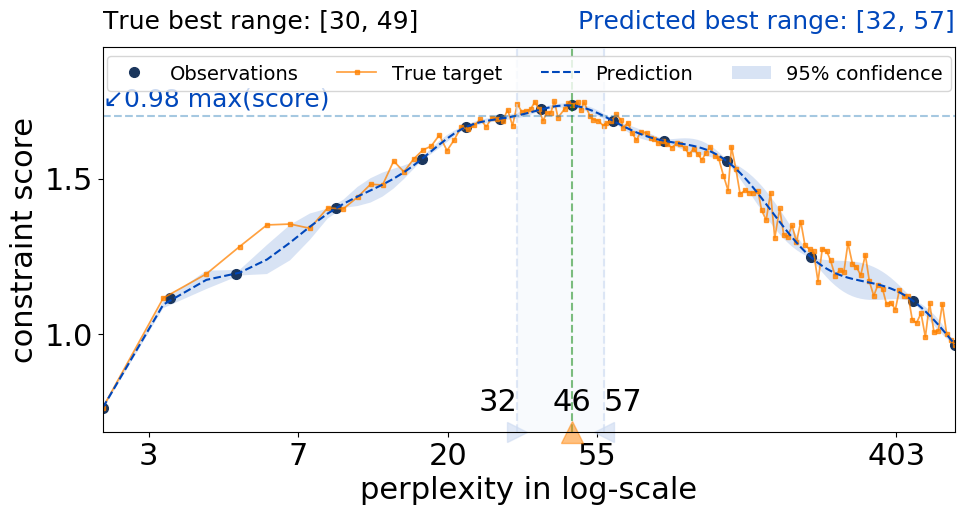
\includegraphics[width=\linewidth]{DIGITS_tsne_bo.png}
        \caption{\emph{DIGITS}}
    \end{subfigure}
    ~
    \begin{subfigure}[b]{.46\linewidth}
        \centering
        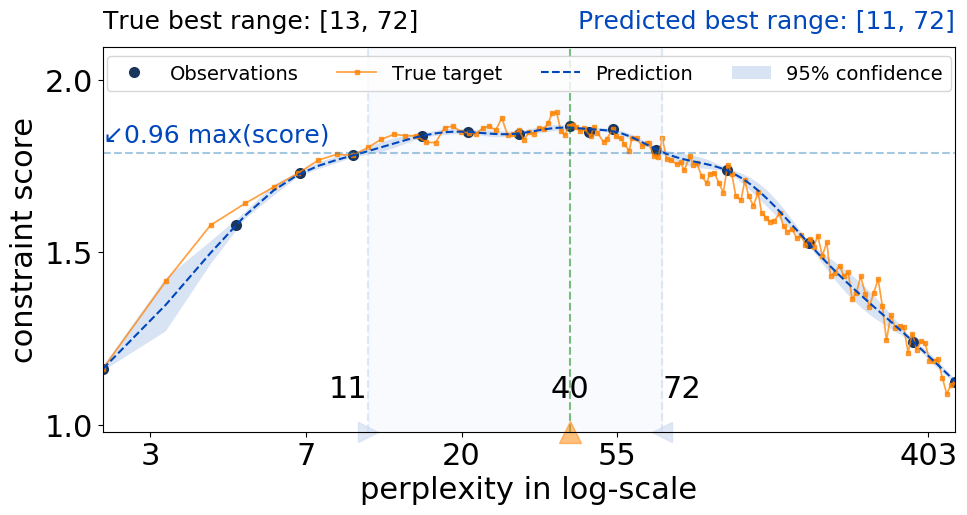
\includegraphics[width=\linewidth]{COIL20_tsne_bo.png}
        \caption{\emph{COIL20}}
    \end{subfigure}
    \vfill
    \begin{subfigure}[b]{.46\linewidth}
        \centering
        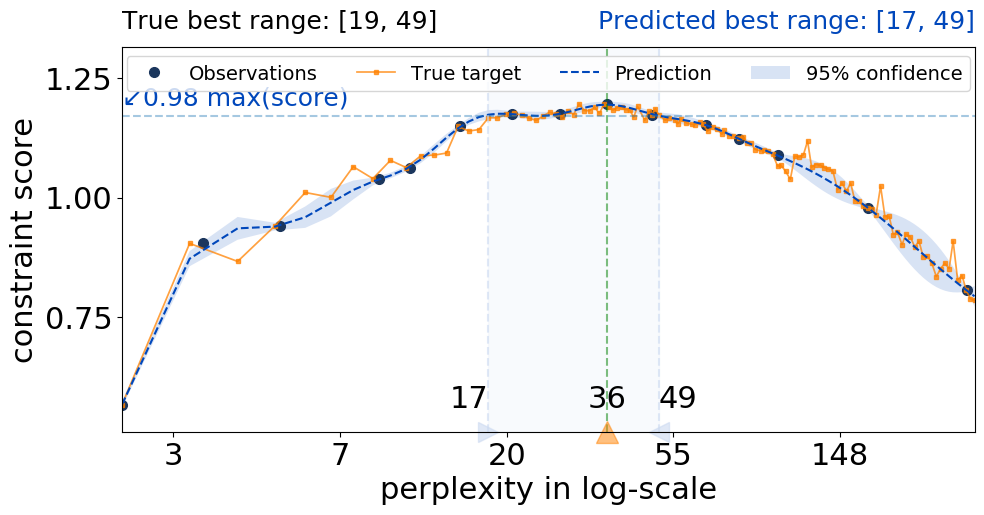
\includegraphics[width=\linewidth]{FASHION1000_tsne_bo.png}
        \caption{\emph{FASHION\_1K}}
    \end{subfigure}
    ~
    \begin{subfigure}[b]{.46\linewidth}
        \centering
        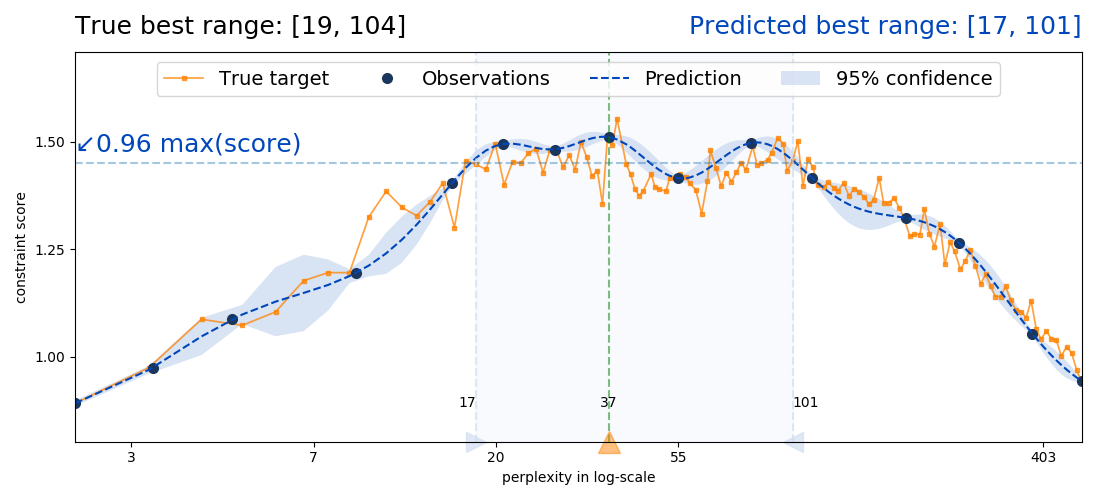
\includegraphics[width=\linewidth]{FASHION_MOBILENET_tsne_bo.png}
        \caption{\emph{FASH\_MOBI}}
    \end{subfigure}
    ~
    \vfill
    \begin{subfigure}[b]{.46\linewidth}
        \centering
        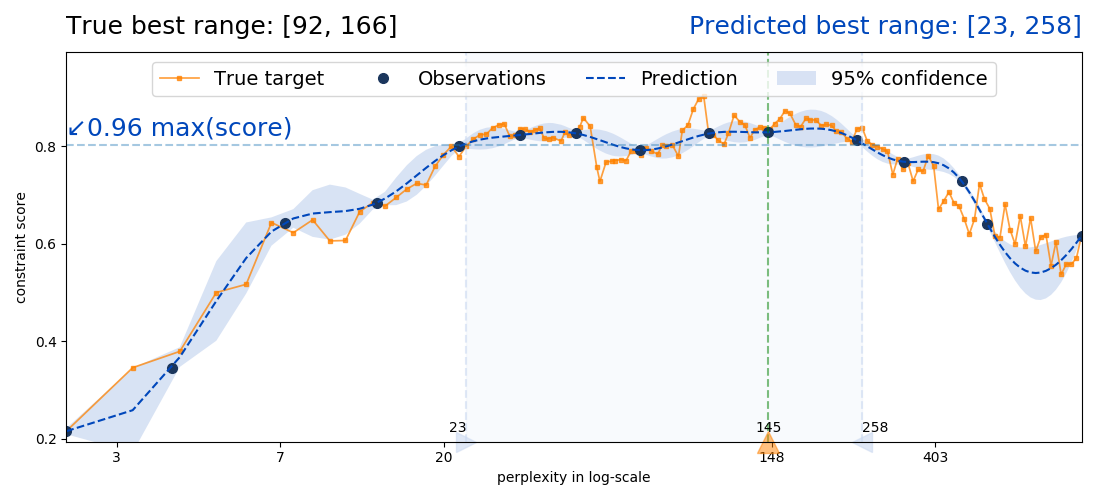
\includegraphics[width=\linewidth]{20NEWS5_tsne_bo.png}
        \caption{\emph{5NEWS}}
    \end{subfigure}
    ~
    \begin{subfigure}[b]{.46\linewidth}
        \centering
        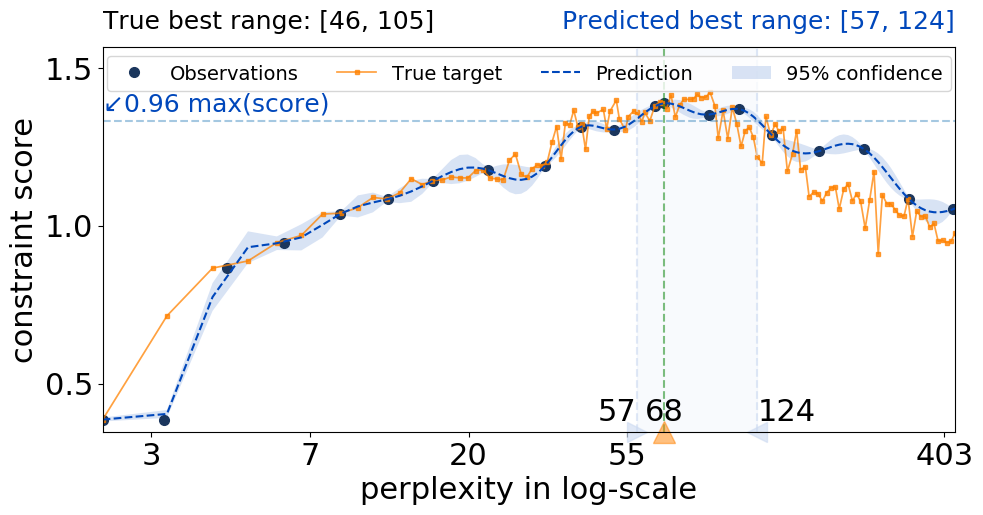
\includegraphics[width=\linewidth]{NEURON_1K_tsne_bo.png}
        \caption{\emph{NEURON\_1K}}
    \end{subfigure}
    \caption{BayOpt approach for  t-SNE}
    \label{fig:tsne:bo:all}
\end{figure}

Fig.~\ref{fig:tsne:bo:all} demonstrates how BayOpt works for tuning t-SNE's perplexity for all six selected datasets.
As proved empirically in the previous section, 10 labeled instances for each class suffice for a stable score.
The scores calculated for all sampled perplexity values ($\in [2, N/3]$, with $N$ is number of instances in a dataset) are used as ground truth.
For all datasets of various size (from 1000 to around 3000 data points), we only need to evaluate the score values for 15 selected perplexities.
These points are selected by BayOpt iteratively, starting with five perplexities randomly initialized.
The score value for each perplexity $p_i$ is calculated and all the pairs $(p_i, f_{score}(p_i))$ are used to train the underlying GP model of BayOpt.
The next predicted perplexity to evaluate is the most promising value according to the GP model that can have a higher $f_{score}$.
When the new perplexity is evaluated, BayOpt gets the new score value and update it's GP model.
More detail and visual explanation on how BayOpt works with the proposed score function can be found in the Appendix~\ref{app:x}.

It should note that, BayOpt does approximate the score function but tries to find its maximum value instead.
The best predicted perplexity range where the predicted score is superior to 96\% of the maximum predicted score is highlighted.
BayOpt with the $f_{score}$ target function converges quickly, only after dozen of iterations.
Fig.~\ref{fig:tsne:bo:all} shows the best prediction at convergence state of BayOpt for all datasets after 15 iterations.
BayOpt does not only find the best hyperparameter but also indicate the region in which it is not certain about its prediction.
This is usually the region of high perplexity values where the $f_{score}$ has large distortion.
Instead of evaluating the score functions for all values of perplexity, BayOpt framework can intelligently choose a limited number of potential perplexities to evaluate and assures to always find a global maximum.

% \subsubsection*{Compare $f_{score}$, $AUC_{log}RNX$ and BIC-based score}
\begin{figure}[]%[pos=h]
    \centering
    \begin{subfigure}[b]{0.3\linewidth}
        \centering
        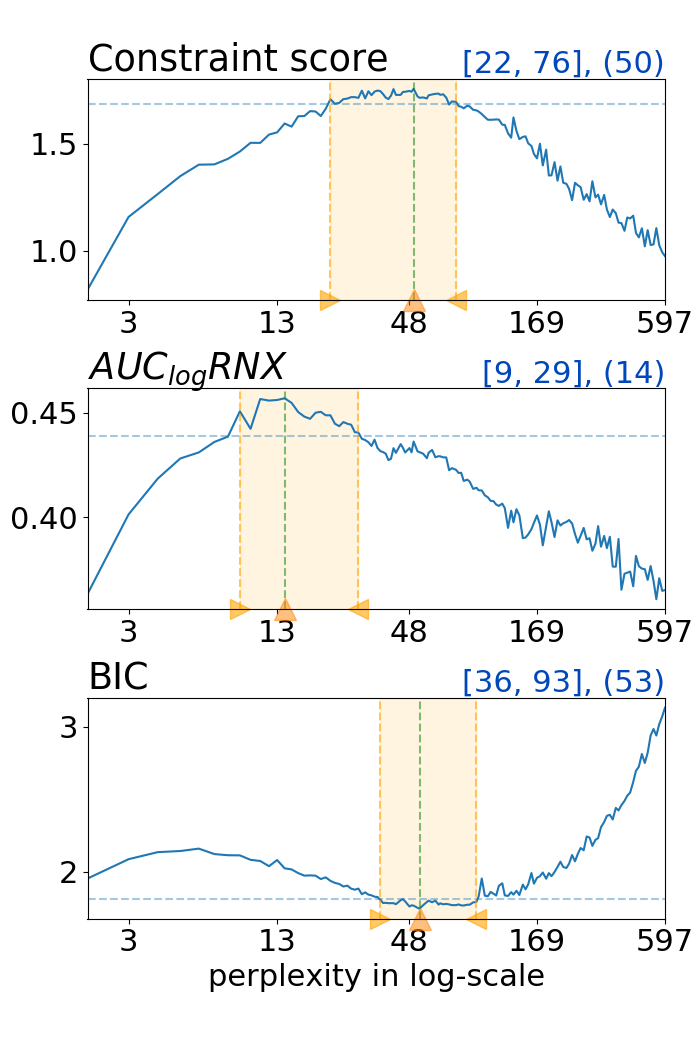
\includegraphics[width=\linewidth]{DIGITS_tsne_compare_scores}
        \caption{DIGITS}
    \end{subfigure}
    ~
    \begin{subfigure}[b]{0.3\linewidth}
        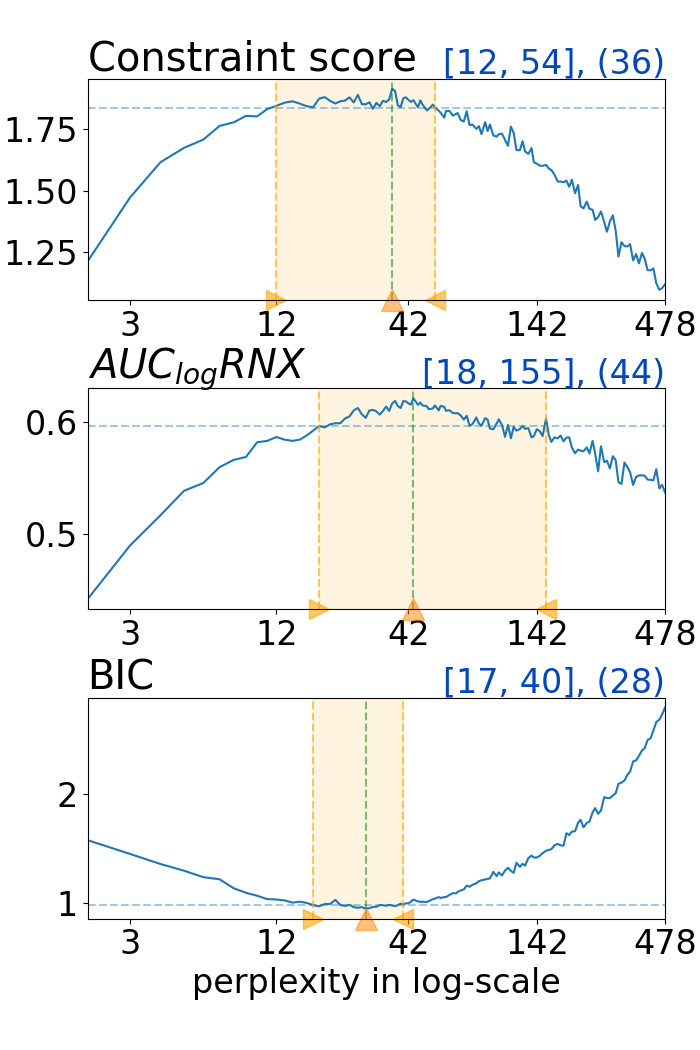
\includegraphics[width=\linewidth]{COIL20_tsne_compare_scores}
        \caption{COIL20}
    \end{subfigure}
    ~
    \begin{subfigure}[b]{0.3\linewidth}
        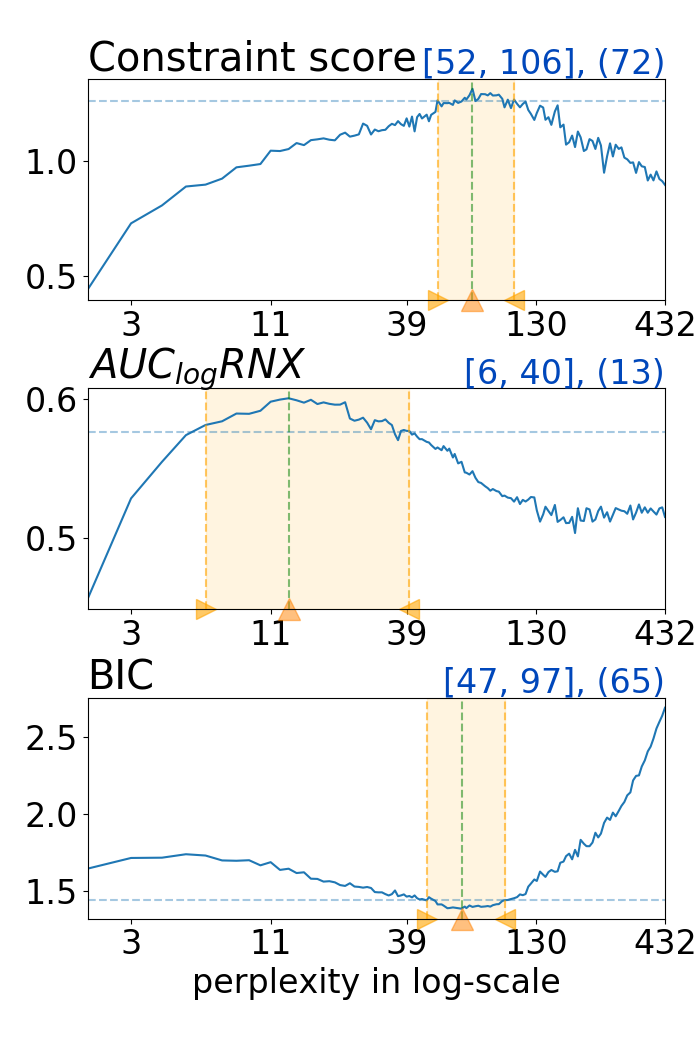
\includegraphics[width=\linewidth]{NEURON_1K_tsne_compare_scores}
        \caption{NEURON\_1K}
    \end{subfigure}
    \vfill
    \begin{subfigure}[b]{0.3\linewidth}
        \centering
        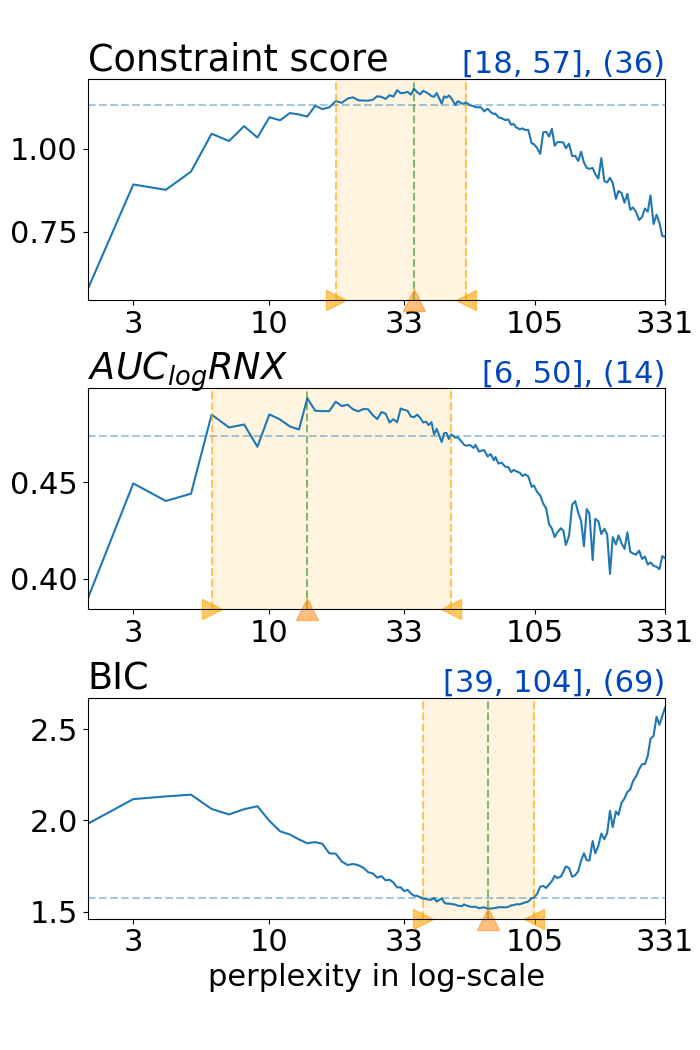
\includegraphics[width=\linewidth]{FASHION1000_tsne_compare_scores}
        \caption{FASHION\_1K}
    \end{subfigure}
    ~
    \begin{subfigure}[b]{0.3\linewidth}
        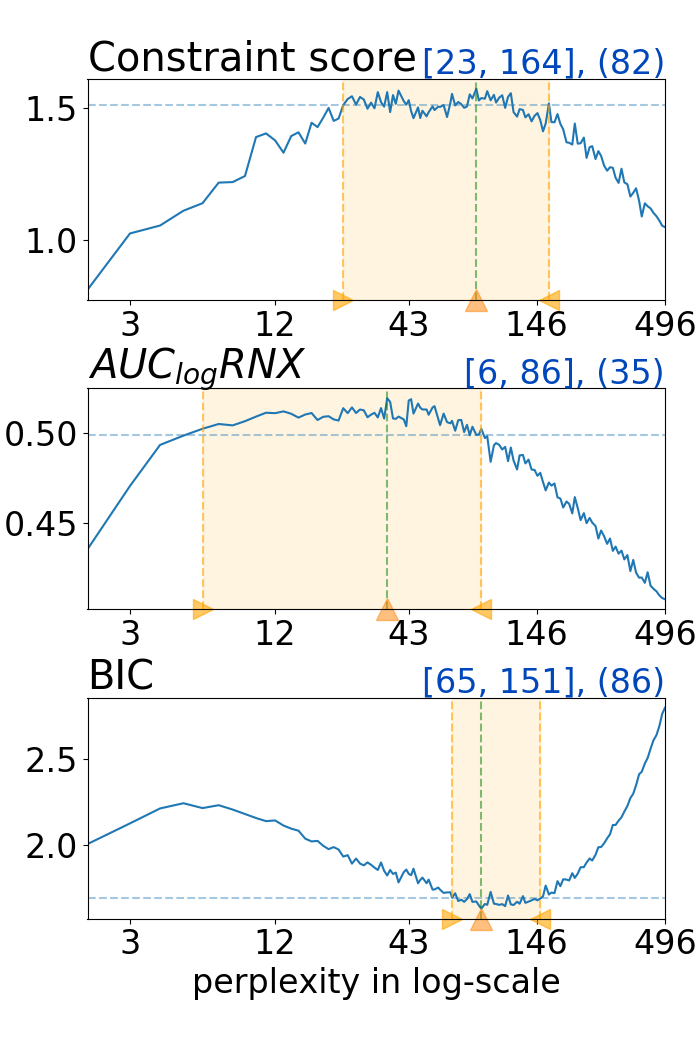
\includegraphics[width=\linewidth]{FASHION_MOBILENET_tsne_compare_scores}
        \caption{FASH\_MOBI}
    \end{subfigure}
    ~
    \begin{subfigure}[b]{0.3\linewidth}
        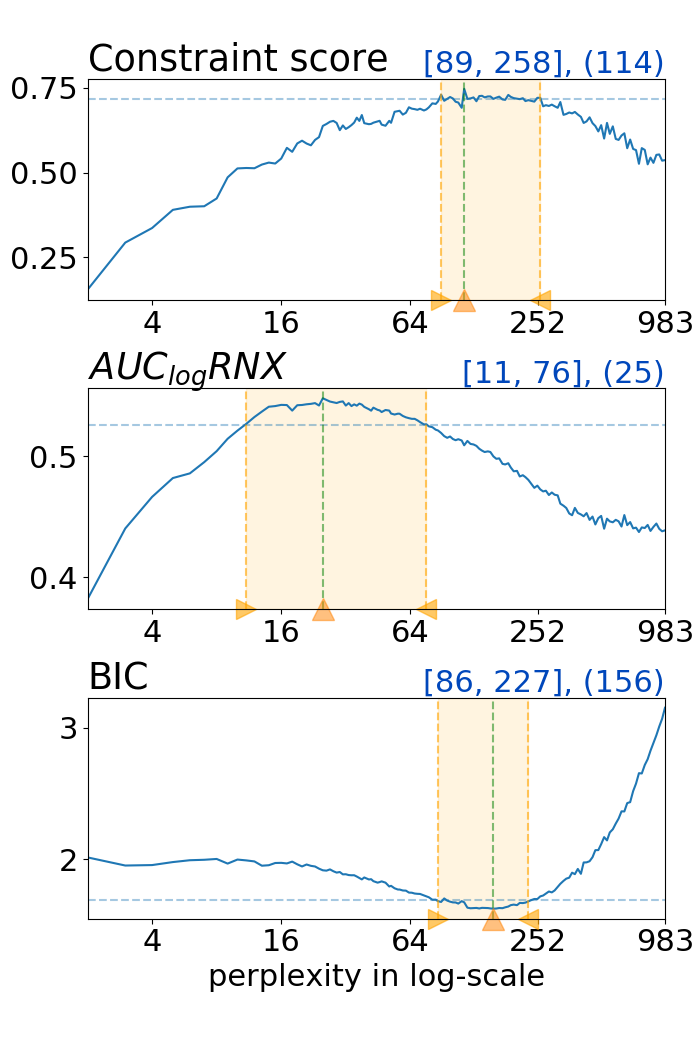
\includegraphics[width=\linewidth]{20NEWS5_tsne_compare_scores}
        \caption{5NEWS}
    \end{subfigure}
    \caption{Comparison of constraint score, $AUC_{log}RNX$ score and BIC score for t-SNE's embeddings.}
    \label{fig:tsne:compare}
\end{figure}

% hardcoded position of figure for t-SNE-{Metamaps and Visualizations}
\begin{figure*}[]%
    \centering
    \begin{subfigure}[b]{.8\linewidth}
        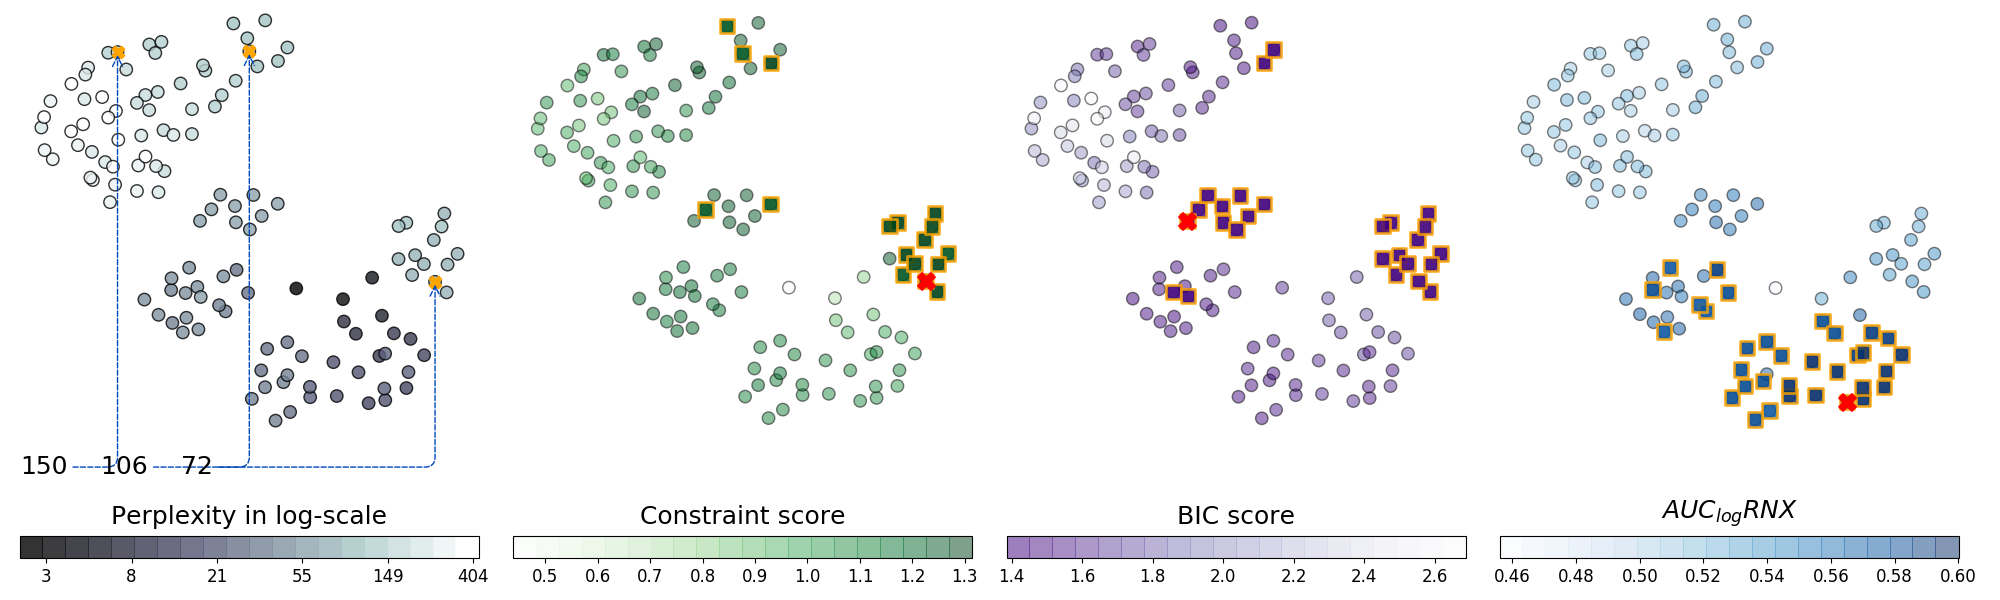
\includegraphics[width=\linewidth]{NEURON_1K_tsne_metamap}
    \end{subfigure}
    ~
    \begin{subfigure}[b]{.8\linewidth}
        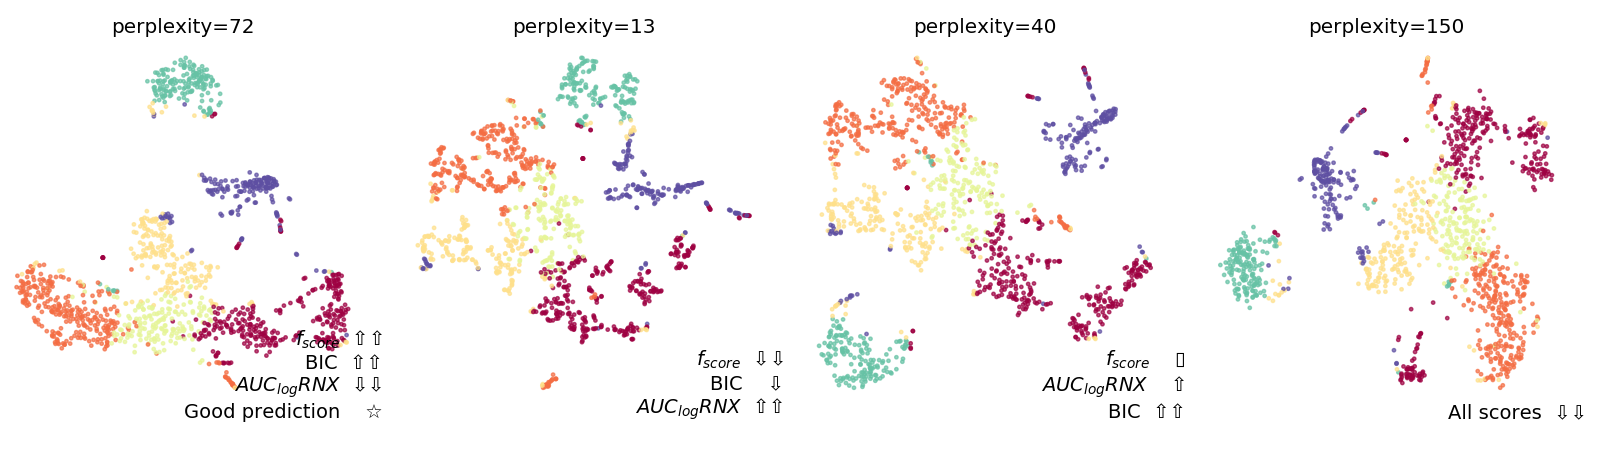
\includegraphics[width=\linewidth]{NEURON_1K_tsne_show}
    \end{subfigure}
    \caption{Metamap and sample visualizations for the selected parameters for \emph{NEURON\_1K} dataset.}
    \label{fig:tsne:meta:NEURON1K}
\end{figure*}

Fig.~\ref{fig:tsne:compare} illustrates the best perplexity range found by $f_{score}$, $AUC_{log}RNX$ and BIC-based score for six datasets.
$f_{score}$ agrees with both $AUC_{log}RNX$ and BIC-based scores in \emph{COIl20}, \emph{FASH\_MOBI} datasets.
$f_{score}$ agrees only with $AUC_{log}RNX$ but not BIC-based score in \emph{FASHION\_1K} dataset.
And $f_{score}$ agrees only with BIC-based score but not $AUC_{log}RNX$ score in \emph{NEURON\_1K}, \emph{5NEWS} and \emph{DIGITS} datasets.
This result suggest that, $f_{score}$ can be used in complement with other quality scores.

% \subsubsection*{Metamaps and Visualizations}
% See figure above
As a proof of concept, the embeddings with all integer values of perplexity are calculated.
A metamap is used in order to visualize the solution space of t-SNE, i.e., to represent all the embeddings with different perplexities.
In this metamap, each point is an embedding corresponding to one perplexity.
The metamap is constructed by applying a visualization method (t-SNE or UMAP) on the ensemble of pre-calculated embeddings.
The metamaps presented in this section are built by UMAP with \emph{n\_neighbors} = 50 and \emph{min\_dist} = 0.1.
The large value of \emph{n\_neighbors} is to reveal the global structure, i.e, the relation of all embeddings in a general view.
An example of metamap for the \emph{NEURON\_1K} dataset and sample visualizations are shown in Fig.~\ref{fig:tsne:meta:NEURON1K}.
(See Appendix~\ref{app:x} for another metamap and sample visualizations of the \emph{DIGITS} dataset).
In this figure, some selected perplexity values are indicated in the first metamap and the corresponding visualizations are shown below.
The second, third and fourth metamaps are colored by the values of $f_{score}$, $AUC_{log}RNX$ and BIC-based score respectively.
The embeddings with high score (superior than 96\% of maximum score) are also highlighted.
In this way, we discover the different regions of best results according different quality scores.
The real world \emph{NEURON\_1K} dataset is selected because the three evaluated scores discover different region in the solution space (visualized by the metamap), which help us observe the structure of the dataset under different aspects.

The sample visualizations in Fig.~\ref{fig:tsne:meta:NEURON1K} served for a qualitative evaluation of the best visualization found by different score.
They are also ranked quantitatively/objectively by its score values as: very preferred ($\Uparrow\Uparrow$), preferred ($\Uparrow$), good enough ($[]$), not preferred ($\Downarrow$) and unfavorable ($\Downarrow\Downarrow$).
The good visualization predicted by BayOpt (whose the tuned hyperparameter in the best predicted range) is denoted by star symbol ($\star$).
As indicated by Wattenberg et. al.~\cite{wattenberg2016use}, we may need more than one plot to understand the hidden pattern in the data.
As suggested by different scores, we can easily discover different region in the solution space and thus discover different structures in the data for which one score can not reveal them all.


%%%%%%%%%%%%%%%%%%%%%%%%%%%%%%%%%%%%%%%%%%%%%%%%%%%%%%%%%%%%%%%%%%%%%%%%%%%%%%%%%%%%%%%%%%%%%%%
\subsection{BayOpt for Tuning Two Parameters of UMAP}
UMAP has not only a solid theoretically foundations in manifold learning but also is very practical with a well documented guide on its hyperparameters \cite{mcinnes2018umap-software}.
The first hyperparameter \emph{n\_neighbors} plays the same role as perplexity for t-SNE and LargeVis, which controls how to reveal local versus global structures in the data.
\emph{n\_neighbors} affects the construction of the k-neighbor graph.
A small value thus leads to many small connected components in the visualization while a large value loses the fine local structure details but give a boarder view of the data.
A suggested range for \emph{n\_neighbors} is $[5, 50]$, with a choice of 10 to 15 being a sensible default.
On the other hand, the second hyperparameter \emph{min\_dist} affects directly the output since it controls how tightly points are packed together and thus is considered to be more important than other hyperparameters for visualization purpose~\cite[Sec.4.3]{mcinnes2018umap}.
The recommended range is $[0.001, 0.5]$ and a reasonable default is 0.1.
Finding the best combination of these two hyperparameters for a specified dataset is hard.
A naive approach requires thousands of evaluation for all discrete combinations.
As a proof of concept, we evaluate $f_{score}$ and $AUC_{log}RNX$ score for all UMAP embeddings on a grid of around 150 integer values for \emph{n\_neighbors} $\in [2, N/3]$ (depending the size of the dataset) and 10 real values for \emph{min\_dist} $\in [0.001, 1]$ in natural logarithmic domain.

\begin{figure}[]%[pos=h]
    \begin{subfigure}[b]{.78\linewidth}
        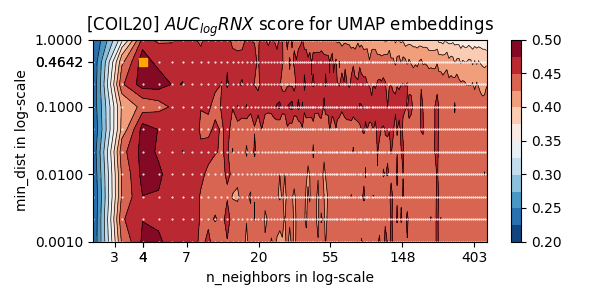
\includegraphics[width=\textwidth]{COIL20_umap_auc_rnx}
        \caption{$AUC_{log}RNX$ score.}
    \end{subfigure}
    ~
    \begin{subfigure}[b]{.78\linewidth}
        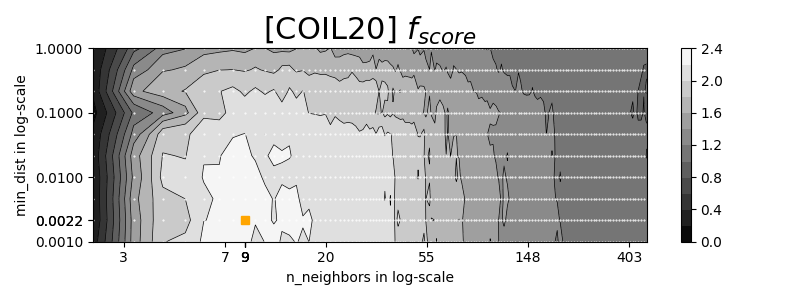
\includegraphics[width=\textwidth]{COIL20_umap_qij_score}
        \caption{$f_{score}$}
    \end{subfigure}
    ~
    \begin{subfigure}[b]{\linewidth}
        \centering
        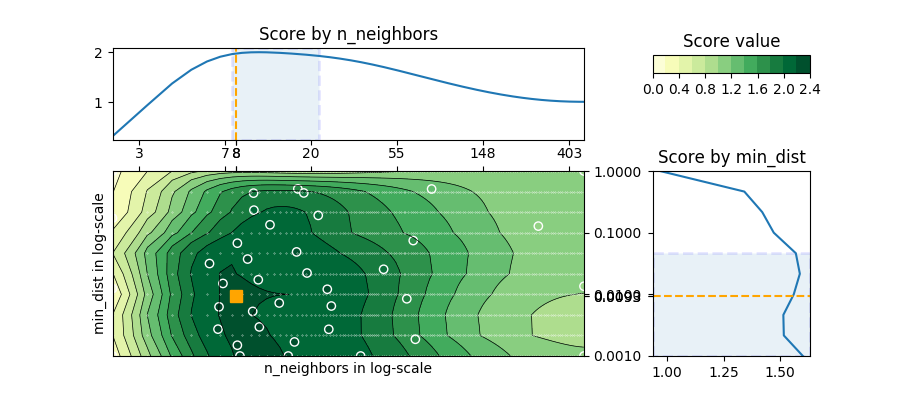
\includegraphics[width=\textwidth]{COIL20_umap_predicted_score}
        \caption{BayOpt predicted score}
    \end{subfigure}
    ~
    \caption{BayOpt for tuning two hyperparameter of UMAP for \emph{COIL20} dataset.}
    \label{fig:bo:umap:COIL20}
\end{figure}

Fig.~\ref{fig:bo:umap:COIL20}(a, b) show $AUC_{log}RNX$ and constraints scores of every combination of hyperparameters on the sample grid for the \emph{COIl20} dataset.
The \emph{COIL20} dataset contained only 20 objects but under different rotations, which gives a very good example for the trade-off of how the local versus global structures are preserved in the visualization. (Some sample visualizations are in Fig.~\ref{fig:umap:meta:COIL20}).
$AUC_{log}RNX$ can not investigate the relevant of the two hyperparameters, as indicated by the homogeneous zone on the left and on top of Fig.~\ref{fig:bo:umap:COIL20}(a).
Indeed, when \emph{n\_neighbors} is small (between 3 and 8), \emph{min\_dist} does not have strong affect. And when \emph{min\_dist} is large enough (larger than 0.1), \emph{n\_neighbors} does not have strong affect either.
In contrast, it is clear that $f_{score}$ in Fig.~\ref{fig:bo:umap:COIL20}(b) can identify a small, reasonable zone of the good hyperparameters.

\begin{figure*}
    \centering
    \begin{subfigure}[b]{.8\linewidth}
        \centering
        \includegraphics[width=\linewidth]{{COIL20_umap_metamap}.png}
    \end{subfigure}
    ~
    \begin{subfigure}[b]{.8\linewidth}
        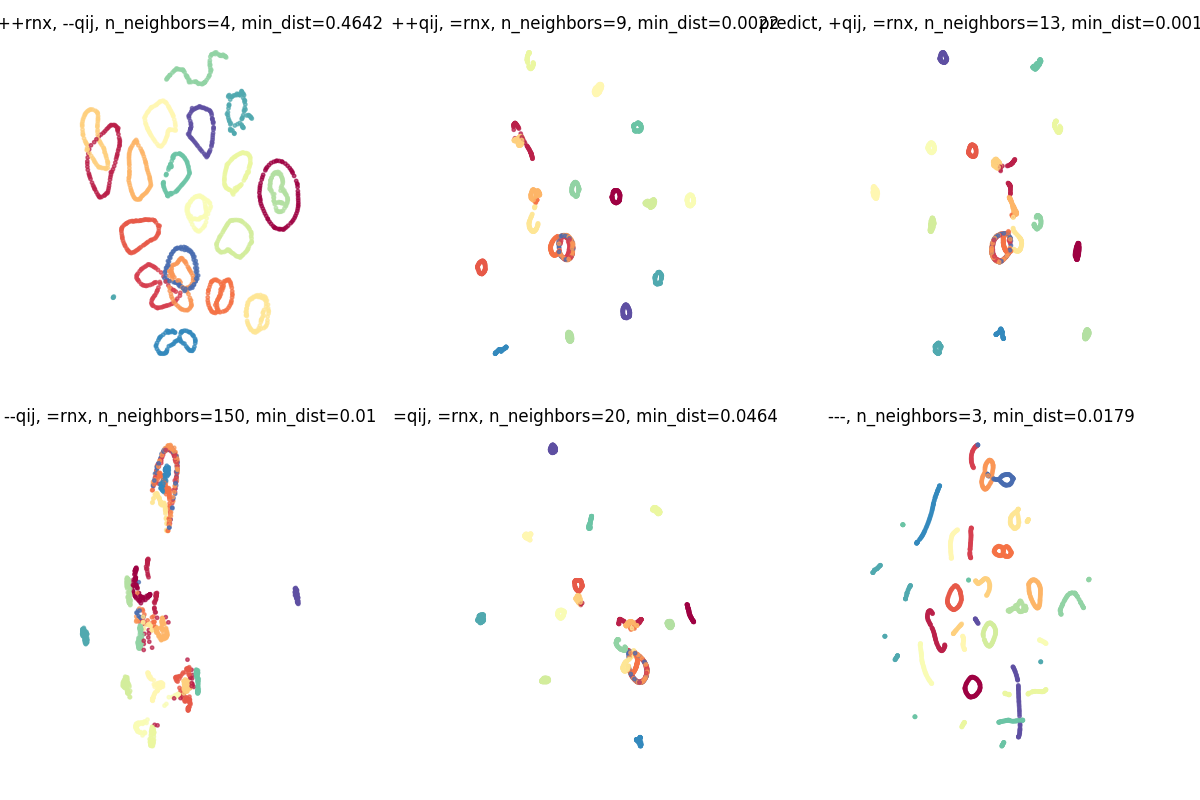
\includegraphics[width=\linewidth]{COIL20_umap_show}
    \end{subfigure}
    \caption{Metamaps and sample visualizations with selected hyperparameters for the \emph{COIL20} dataset.}
    \label{fig:umap:meta:COIL20}
\end{figure*}

The predicted best hyperparameter combination is illustrated in Fig.~\ref{fig:bo:umap:COIL20}(c).
Under BayOpt framework, only 40 combinations are selected and evaluated to find the best \emph{n\_neighbors} = 8 and \emph{min\_dist} = 0.01 for UMAP instead of evaluating more than 1000 combination in the sample grid.
The predicted optimal hyperparameters are close to the ground truth optimum (\emph{n\_neighbors} = 9 and \emph{min\_dist} = 0.0022) despite a very limited number of evaluation.

TODO:
Intro to metamap and sample vis in Fig.~\ref{fig:umap:meta:COIL20}.

%%%%%%%%%%%%%%%%%%%%%%%%%%%%%%%%%%%%%%%%%%%%%%%%%%%%%%%%%%%%%%%%%%%%%%%%%%%%%%%%%%%%%%%%%%%%%%%
%%%%%%%%%%%%%%%%%%%%%%%%%%%%%%%%%%%%%%%%%%%%%%%%%%%%%%%%%%%%%%%%%%%%%%%%%%%%%%%%%%%%%%%%%%%%%%%
\section{Flexibility of the Proposed Score}\label{sec:result:flexibility}

QUESTION here...

$AUC_{log}RNX$ metric evaluates how the neighborhood information is preserved.
The BIC-based score evaluates the trade-off between KL loss and the value of perplexity in t-SNE.
In contrast, the $f_{score}$ evaluates how the constraints are preserved based on the external input of labeled instances.
Naturally, the constraints generated from the class labels reflect the class-relationship between the data points in the same class.
% However, if we have another subset of \emph{`semantic'} labels

Demo score's flexibility for \emph{FASH\_MOBI}(Fig.~\ref{fig:flex:fashionmobilenet}), \emph{5NEWS} (Fig.~\ref{fig:flex:5news}) and \emph{NEURON\_1K} (Fig.~\ref{fig:flex:neuron}).

\begin{figure*}%[pos=h]
    \centering
    \includegraphics[width=.8\linewidth]{{FASHION_MOBILENET_score_flexibility}.png}
    \caption{Flexibility of $f_{score}$ for \emph{FASH\_MOBI} dataset}
    \label{fig:flex:fashionmobilenet}
\end{figure*}

\begin{figure*}%[pos=h]
    \centering
    \includegraphics[width=.8\linewidth]{{20NEWS5_score_flexibility}.png}
    \caption{Flexibility of $f_{score}$ for \emph{5NEWS} dataset}
    \label{fig:flex:5news}
\end{figure*}

\begin{figure*}%[pos=h]
    \centering
    \includegraphics[width=.8\linewidth]{{NEURON_1K_score_flexibility}.png}
    \caption{Flexibility of $f_{score}$ for \emph{NEURON\_1K} dataset}
    \label{fig:flex:neuron}
\end{figure*}


%%%%%%%%%%%%%%%%%%%%%%%%%%%%%%%%%%%%%%%%%%%%%%%%%%%%%%%%%%%%%%%%%%%%%%%%%%%%%%%%%%%%%%%%%%%%%%%
%%%%%%%%%%%%%%%%%%%%%%%%%%%%%%%%%%%%%%%%%%%%%%%%%%%%%%%%%%%%%%%%%%%%%%%%%%%%%%%%%%%%%%%%%%%%%%%
\section{Discussion and Future Work}

principle contribution: propose a flexible score which is independent to DR methods and integrate into BayOpt framework.

\subsubsection*{Powerful methods still need hyperparameter tuning.}
t-SNE, LargeVis and UMAP are widely used since they make reasonable visualizations in which data points in the same class are placed close together.
In this way, the neighborhood information is preserved and the local structure of the data is highlighted.
However, as pointed out in the article ``How to use t-sne effectively''~\cite{wattenberg2016use}, \emph{the distance between clusters in t-SNE embedding might not mean anything}.
That means in t-SNE embeddings, sometimes the very related or similar groups are placed far apart while unrelated or different groups are placed close together.
The reason is that, t-SNE can not to preserve the distance in the data and it also does not guarantee to preserve much global structure either.
In contrast, UMAP introduces \emph{min\_dist} hyperparameter to control how tightly the connected components appear in the visualization.
By using a small \emph{min\_dist}, one can expect the small concentrated groups in the visualization are well isolated.


\subsubsection*{The proposed constraint preserving score is a flexible function.}
+ works well
+ change input constraint
+ change function form (triplet, contrastive)

\subsubsection*{Constraint generation and Visualization Evaluation}
+ Auto or user

\subsubsection*{Advantage of BayOpt}

\par
Discuss the variance of the proposed score (w.r.t to different set of constraints, different number of constraints).
Say, the constraint-based score is a stochastic function.
Say, how BayOpt can take into account the uncertainty (the variance of the score) to estimate the maximum of this stochastic function.


\par
The violated constraints in our methods correspond to the shortcoming of t-SNE in \cite{wattenberg2016use}.
t-SNE can not preserve the within-cluster distances and between-clusters distances.
[TODO: Add reproduced figures].
The $q_{ij}$-based score can help to understand the defective of the visualization.

\par
Add discussion for UMAP.

\par
Easily generate pairwise constraints from labels.
  Only need small amount of labeled points for each class to generate hundreds of constraints.
  The proposed method only need 200 constraints to work well.
  [TODO: Test with smaller number of constraints to see if it works. 200 constraints seem too much].

\par
Can replace the auto-generated constraints by the manual constraints of the real user.

\par
The user can interact directly in the loop of Bayesian Optimization method to select the next hyperparameter to discover.


\par
Both the constraint-based score and the BayOpt's internal steps are explainable even for the non-technical users.

\vspace{8pt}
\par (4) Future work:

(a) User experiment:

+ Integrate the user's feedback in two stages of our workflow.
The users can select the pairwise constraints or label some points (used to generate the constraints) to build the score.
They can also manually select the next hyperparameters to evaluate in a customized interactive BayOpt framework.

+ Take the preference of the users on the presented visualizations to evaluate the quality of the visualization. We search for if the best visualization selected by the user corresponds to the result of our method.


(b) Integrate directly the pairwise constraints into the optimization process of BayOpt.
BayOpt is now used as a generic toolbox to find the extreme of a blackbox costly objective function.
Our idea is to use the pairwise constraint to modify the kernel in the covariance function of Gaussian Process model, which is the core element of BayOpt.


%%%%%%%%%%%%%%%%%%%%%%%%%%%%%%%%%%%%%%%%%%%%%%%%%%%%%%%%%%%%%%%%%%%%%%%%%%%%%%%%%%%%%%%%%%%%%%%
%%%%%%%%%%%%%%%%%%%%%%%%%%%%%%%%%%%%%%%%%%%%%%%%%%%%%%%%%%%%%%%%%%%%%%%%%%%%%%%%%%%%%%%%%%%%%%%
\section{Conclusion}

\par (1) Repeat the problem of hyperparameter tuning for DR methods and our solution:

+ The proposed constraint-based score is independent to how the embedding is produced and can be used with any DR methods.
This score is built upon a limited number of constraints but can distinguish the visualizations preferring local structure and those preferring global structure.

+ A finding that Bayesian Optimization approach fits well in our problem.


\vspace{8pt}
\par (2) Summary the advantages of the two above elements

+ The constraint-based score agree the the well-known quality metric.

+ This score can be visually represented to explain the violated pairs.

+ By combining this score with BayOpt approach, we can tune many hyperparameters at the same time for many widely used DR methods like t-SNE or UMAP.

+ BayOpt takes into account the uncertainty in the score values and also explainable. We can observe the internal optimization step to answer the question: why to choose the next promising hyperparameters to try?

The hyperparameters of t-SNE and UMAP make these methods difficult to use correctly but also make them flexible.
These methods can produce different visualizations and reveal different hidden structures in the data.
To evaluate the embedding quality of such flexible methods, we need a flexible score.
The state of the art $AUC_{log}RNX$ metric or the BIC-based score has no flexibility to capture different visualization results.